\documentclass[pdf]{beamer}
\usepackage[utf8]{inputenc}
\usefonttheme{professionalfonts}
\usetheme{Madrid}
\useoutertheme{shadow}
\useinnertheme{circles} %Less sharpened edges
\usecolortheme{}
\title{Advanced Complexity : Fundamentals}
\author{Marius}
\date{October 2021}

\usepackage{stmaryrd}   %N
\usepackage{esvect}     %Vector
\usepackage{hyperref}   %hypertext link
\usepackage{graphicx}
\usepackage{amsmath}    %overset
\usepackage{amssymb}    %square
\usepackage{amsthm}     %proof
\usepackage{xcolor}     %color
\usepackage{esvect}     %Vector
\usepackage{tikz}       %draw
\usetikzlibrary{positioning}
\usetikzlibrary{automata}
\usetikzlibrary{arrows}


%%% Operator %%%
\newcommand{\norm}[1]{\left\Vert #1 \right\Vert}
\newcommand{\card}[1]{\ensuremath{\left\|#1 \right\|}}
\newcommand{\interval}[2]{\ensuremath{\llbracket #1, \; #2 \rrbracket}}
\newcommand{\set}[1]{\{ #1 \}}
\newcommand{\br}[1]{\ensuremath{\llbracket #1 \rrbracket}} %Interpretation
\newcommand{\floor}[1]{\lfloor #1 \rfloor}
\newcommand{\ceil}[1]{\lceil #1 \rceil}
\newcommand{\ol}[1]{\overline{#1}}
\newcommand{\ul}[1]{\underline{#1}}

% Shortcuts sets
\newcommand{\bb}[1]{\mathbb{#1}}
\newcommand{\mc}[1]{\mathcal{#1}} %Abrev mathcal
\newcommand{\N}{\ensuremath{\mathbb{N}}}
\newcommand{\Z}{\ensuremath{\mathbb{Z}}}
\newcommand{\Q}{\ensuremath{\mathbb{Q}}}
\newcommand{\C}{\ensuremath{\mathbb{C}}}

%%% shorcuts logic %%%
\newcommand{\G}{\Gamma} % Abreviation pour logique etc..
\newcommand{\D}{\Delta} % Abreviation pour logique
\newcommand{\T}{\mathcal{T}} %Abreviation T pour logique

\renewcommand{\O}{\mathcal{O}}
\newcommand{\V}{\mathcal{V}}
\newcommand{\A}{\mathcal{A}}
\newcommand{\R}{\mathcal{R}}
\begin{document}
\maketitle
\begin{frame}
\frametitle{A brief overview}

 
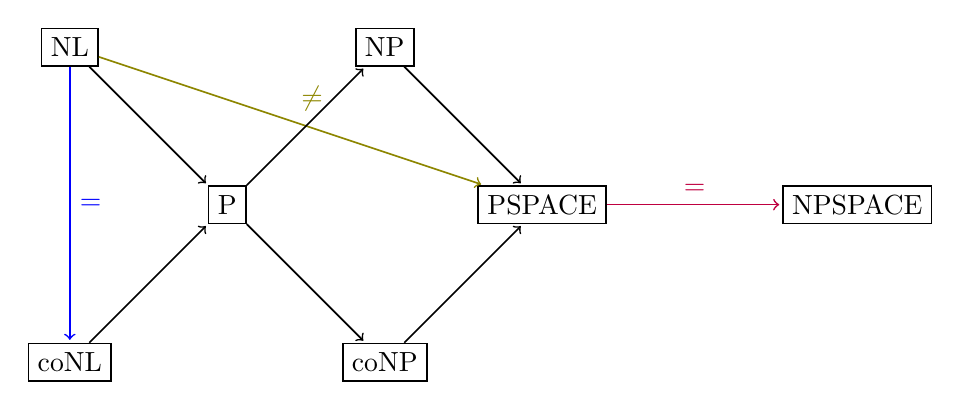
\begin{tikzpicture}[->,shorten >=1pt,auto,node distance=3cm,semithick]
 
    \node[rectangle,draw] at (0,0) (nls)  {NL};
    \node[rectangle,draw] at (0,-4) (conls) {coNL};
    \node[rectangle,draw] (pt) at (2,-2) {P};
    \node[rectangle,draw] (npt)  at (4,0) {NP};
    \node[rectangle,draw] (conpt) at (4,-4) {coNP};
    \node[rectangle,draw] (ps) at (6,-2) {PSPACE};
    \node[rectangle,draw] (nps) at (10,-2) {NPSPACE};

    \path (nls)   edge[blue]        node {$=$} (conls)
    (nls)   edge        node {} (pt)
    (nls)   edge[olive]        node {$\neq$} (ps)
    (conls)   edge        node {} (pt)
    (pt)   edge        node {} (npt)
    (pt)   edge        node {} (conpt)
    (npt)   edge        node {} (ps)
    (conpt)   edge        node {} (ps)
    (ps)   edge[purple]        node {$=$} (nps);
 
\end{tikzpicture}

\bigskip
\color{blue} Immerman-Szelepscényi theorem \newline
\color{olive} Strict hierarchy theorem \newline
\color{purple} Savitch theorem \newline


\end{frame}

\begin{frame}
\frametitle{Definitions}

\begin{block}{Fonction propre}
Fonction croissante et calculable en temps $\O(n+f(n))$ et en espace $\O(f(n))$.
\end{block}


\begin{block}{Machine alternantes}
L'espace des états finaux est partitionné entre \emph{existentiel} et \emph{universel}\newline
Une machine accepte un mot depuis un état existentiel s'il existe une exécution acceptante \newline
Une machine accepte un mot depuis un état universer si toute exécution accepte.\newline
\end{block}


\begin{exampleblock}{Intuition}
Une machine alternante peut-ête vue comme un jeu à deux joueurs. \newline
Un mot est accepté ssi le joueur existentiel dispose d'une stratégie gagnante.
\end{exampleblock}
\end{frame}

\begin{frame}
\frametitle{\mc{C}-complete problems}

\begin{block}{A few complete-problems}
$REACH$ is \textbf{NL}-complete \newline 
$QBF$ is \textbf{PSPACE}-complete \newline 
$HORN-SAT$ is \textbf{P}-complete \newline 
$CIRCUIT~VALUE$ is  \textbf{P}-complete \newline 
$MONOTONE~CIRCUIT~VALUE$ is \textbf{P}-complete \newline 
\end{block}


\begin{exampleblock}{Reminders}
A \emph{Horn clause} contains at most one positive literal. \newline
A \emph{Circuit value} is a DAG labelled with $\wedge, \vee, \ol{\wedge}, \ol{\vee}$ \newline
A \emph{Monoton circuit value} is a DAG labelled with $\wedge, \vee$ \newline
\end{exampleblock}

\end{frame}

\begin{frame}
\frametitle{Usual classes of complexity : Major theorems}


\begin{alertblock}{Savitch theorem}
For any proper function $f>\log$, $\mathbf{NSPACE}(f(n)) \subseteq \mathbf{SPACE}(f^2(n))$
\end{alertblock}

\begin{alertblock}{Immerman-Szelepscényi theorem}
$REACH$ is \textbf{coNL}
\end{alertblock}

\begin{exampleblock}{Corollaries (more important)}
$\mathbf{NPSPACE} = \mathbf{PSPACE}$\newline
$\mathbf{NL}=\mathbf{coNL}$
\end{exampleblock}


\end{frame}
\begin{frame}
\frametitle{Relation between TM and ATM}

\begin{block}{A few results}
$\mathbf{AP} = \mathbf{PSPACE}$ (Chandra-Kozen-Stockmeyer I) \newline
$\mathbf{AL} = \mathbf{P}$ (Chandra-Kozen-Stockmeyer II) \newline
$\mathbf{APSPACE} = \mathbf{EXPTIME}$ \newline
\end{block}

\begin{exampleblock}{Corollaries (more important)}
Le temps alternant, c'est de l'espace ! \newline
L'espace alternant, c'est du temps exponentiel ! \newline
\end{exampleblock}

\end{frame}

\begin{frame}
\frametitle{Polynomial hierarchy}

\begin{block}{$\Sigma^p_n$ and $\prod^p_n$}
$\Sigma^p_0=\prod^p_0=\mathbf{P}$\newline
$\Sigma^p_{n+1}$ la classe des langages $L=\{x \vert\exists y \in A* \text{ de taille } p(n), x\#y \in L′\}$\newline
$\prod^p_{n+1}$ la classe des langages $L=\{x \vert\forall y \in A* \text{ de taille } p(n), x\#y \in L′\}$\newline
\end{block}

\end{frame}

\title{Advanced Complexity : Probabilistic classes of complexity}

\begin{frame}
\maketitle
\end{frame}

\begin{frame}
\frametitle{Randomized TM}

\begin{block}{Randomized TM}
A TM augmented with a random tape on read-only and never read twice.
\end{block}

\begin{block}{RP}
A language $L$ is in \textbf{RP} if there is a polynomial RTM such that : \newline
$\bullet$ If $x \in L$ then $\bb{P}(M(x,r)~accepts)>\frac{1}{2}$ \newline
$\bullet$ Otherwise the machine always rejects. \newline
A language $L$ is in \textbf{co-RP} if $L^c \in \mathbf{RP}$
\end{block}

\begin{exampleblock}{RP : A few remarks}
$PRIMALITY$ is in $co-RP$ (Miller-Rabbin)\newline
$\forall \epsilon \in ]0,1[, \mathbf{RP}=\mathbf{RP}(\epsilon)$ \newline
$ ~\rightarrow$ Simulate $\M(x,r)$ for various $r$ and answer the disjunction. \newline
Better : $\forall q(n), \mathbf{RP}=\mathbf{RP}(2^{-q(n)})$ \newline
$\textbf{P} \subseteq  \textbf{RP} \subseteq \textbf{NP}$
\end{exampleblock}
\end{frame}

\begin{frame}
\frametitle{Zero Probability of error Polynomial-time}

\begin{block}{ZPP}
\textbf{ZPP}= \textbf{RP} $\cap$ \textbf{co-RP} \newline
\textbf{ZPP} also languages decidable in average polynomial time with $\bb{P}(M~errs)=0$.
\end{block}

\end{frame}

\begin{frame}
\frametitle{Bounded Probability of error Polynomial time}

\begin{block}{BPP}
A language $L$ is in \textbf{BPP} if there is a polynomial RTM such that : \newline
$\bullet$ If $x \in L$ then $\bb{P}(M(x,r)~accepts)>\frac{2}{3}$ \newline
$\bullet$ Otherwise $\bb{P}(M(x,r)~accepts)<\frac{1}{3}$ \newline
\end{block}

\begin{exampleblock}{BPP}
It would have been good to have an example :) \newline
$\mathbf{BBP}=\mathbf{co-BPP}$\newline
$\forall \epsilon \in ]0,\frac{1}{2}[~ \mathbf{BPP}=\mathbf{BPP}(\epsilon)$ \newline
$ ~\rightarrow$ Simulate $\M(x,r)$ for various $r$ and answer the majority. \newline
Better : $\forall q(n), \mathbf{BPP}=\mathbf{BPP}(2^{-q(n)})$ \newline
\end{exampleblock}
\end{frame}

\begin{frame}
\frametitle{The Sipser-Gàcs-Lautemann Theorem}

\begin{alertblock}{SGC Theorem}
$\mathbf{BPP} \subseteq \Sigma^p_2 \cap \Pi^p_2$
\end{alertblock}

\begin{exampleblock}{A few reminders}
$\Sigma^p_2 = \exists \cdot \mathbf{coNP} = \exists \cdot \forall \cdot \mathbf{NP}$ \newline
$\Pi^p_2 = \mathbf{co-\Sigma^p_2} =\forall \cdot \mathbf{\Sigma^p_2} = \forall \cdot \exists \cdot \forall \cdot \mathbf{NP}$ \newline
\end{exampleblock}


\begin{exampleblock}{Proof draft}
$\bullet~\mathbf{BPP} \subseteq \Sigma^p_2$ \newline
Lautemann's trick : \newline $x \in L$ iif $\{0,1\}^{p(n)}$ coverable by translations of $\{r \vert M(x,r) accepts\}$\newline
This means $x \in L$  if and only if $\exists t_1..t_n \forall r$, one of the $M(x,r+t_i)$ accepts\newline
Hence the result. \newline
$\bullet~\mathbf{BPP} \subseteq \Pi^p_2$ \newline
This is a direct consequence of $\mathbf{BPP} = \mathbf{co-BPP}$
\end{exampleblock}

\end{frame}

\begin{frame}
\frametitle{P/Poly}

\begin{block}{Uniform P/Poly}
A langage L is in \textbf{Uniform P/Poly} if for every $n\in \N$, one can build $C_n$ \newline
$\bullet $ in space $O(\log n)$\newline
$\bullet$ s.t $\forall x$ of size $n$, $\x \in L$ iff $C_n[x]=1$\newline
\end{block}

\begin{block}{P/Poly}
A langage L is in \textbf{P/Poly} if for every $n\in \N$, There is a circuit $C_n$ \newline
$\bullet $ of polynomial size in $n$ \newline
$\bullet$ s.t $\forall x$ of size $n$, $\x \in L$ iff $C_n[x]=1$\newline
The circuits does not need to be actually buildable anymore.
\end{block}

\begin{exampleblock}{Two remarks}
\textbf{P}=\textbf{Uniform P/Poly}\newline
There are \textbf{undecidable problems} in \textbf{P/Poly}.
\end{exampleblock}

\end{frame}

\begin{frame}
\frametitle{Adleman's Theorem}

\begin{alertblock}{Adleman's Theorem}
\textbf{BPP} $\subseteq$ \textbf{P/Poly}
\end{alertblock}

\begin{exampleblock}{Proof Draft}
$L \in \mathbf{P/Poly}$ iff $\exists~\mc{M}$ and $(w_n)_{n\in\N}$ s.t \newline
$\bullet$ advice strings $w_n$ are of polynomial sizes \newline
$\bullet$ $\forall x$ of size $n$, $x \in L$ iff $\mc{M}(x,w_n)$ accepts \newline
First, we prove that there exists $r_n$ such that $\mc{M}(x,r_n)$ always returns the correct answer \newline
Then, we use $r_n$ as advice strings.
\end{exampleblock}

\end{frame}

\begin{frame}
\frametitle{Karp-Lipton Theorems}

\begin{alertblock}{Karp-Lipton Theorems}
\textbf{I.} If \textbf{NP} $\subseteq$ \textbf{P/Poly}, \textbf{PH} collapses at level 2.\newline
\textbf{II.} If \textbf{NP} $\subseteq$ \textbf{P/Poly}, \textbf{PH} $\subseteq$ \textbf{P/Poly}\newline
\end{alertblock}   

\begin{exampleblock}{Reminders}
\textbf{PH} collapsing at level 2 means that $\Sigma^p_2 =\Pi^p_2=...$\newline
By properties of the \textbf{co} operator, it is equivalent to $\Sigma^p_2 \subseteq \Pi^p_2$\newline   
Using Adleman's theorem, \textbf{NP} $\subseteq$ \textbf{BPP} would be a sufficient condition.
\end{exampleblock}

\end{frame}

\begin{frame}
\frametitle{Arthur-Merlin Games (I)}

\begin{block}{\textbf{AM}}
L is in \textbf{AM} iff $\forall g, \exists \text{ poly-time } \A, \text{Merlin map } M \text{ with poly size outputs} \text{ and } D \in \textbf{P}$ s.t \newline
$\bullet$ if $x \in L$, $\bb{P}(x\#\A(x,r)\#r\#M(x\#q\#r)\in \mathbf{D}) \leq  1 - \frac{1}{2^{g(n)}}$ \newline    
$\bullet$ if $x \notin L$, then $\forall M',\bb{P}(x\#\A(x,r)\#r\#M'(x\#q\#r)\in \mathbf{D}) \leq  \frac{1}{2^{g(n)}}$
\end{block}

\begin{exampleblock}{Intuition}
Arthur asks a question to Merlin depending on $x$ and $r$.\newline
Merlin tries to convince Arthur that $x \in L$ with a polynomial answer. \newline
Finally, a polynomial referee must decide wether Merlin was convincing with exponentially low-error.
\end{exampleblock}

\end{frame}

\begin{frame}
\frametitle{Arthur-Merlin Games (II)}

\begin{exampleblock}{Arthur-Merlin Games : A few results}
We can define different classes depending on how many times Arthur and Merlin can interact and the order.\newline
$\mathbf{\epsilon}$ = \textbf{P}\newline
\textbf{A} = \textbf{BPP} \newline
\textbf{M} = \textbf{NP}\newline
\textbf{MA},\textbf{AM}...
\end{exampleblock}
\end{frame}


\begin{frame}
\frametitle{Interactive Proofs}

\begin{block}{\textbf{IP}}
L is in \textbf{IP} iff $\forall g, \exists \text{ poly-time } \A, \text{Merlin map with poly size outputs } M \text{ and } D \in \textbf{P}$ s.t \newline
$\bullet$ if $x \in L$, $\bb{P}(x\#\A(x,r)\#r\#M(x\#q) \in \mathbf{D}) \leq  1 - \frac{1}{2^{g(n)}}$ \newline    
$\bullet$ if $x \notin L$, then $\forall M',\bb{P}(x\#\A(x,r)\#r\#M'(x\#q)\in \mathbf{D}) \leq  \frac{1}{2^{g(n)}}$
\end{block}


\begin{exampleblock}{Intuition}
We proceed in the same fashion as before but Merlin does not have access to the random tape $r$ anymore.\newline
Note that Arthur can still send $r$ as part of the question, hence \textbf{AM} $\subseteq$ \textbf{IP}
\end{exampleblock}
\end{frame}


\begin{frame}
\frametitle{The Graph Isomorphism Problem}

\begin{block}{GI}
D : Two graphs $G$ and $G'$ \newline
Q : Are they isomorphic ? \newline
\end{block}

\begin{alertblock}
$GNI = coGI \in \mathbf{IP}$
\end{alertblock}
\end{frame}

\begin{frame}
\frametitle{BP operator}


\begin{block}{BP$\cdot\mc{C}$}
As a generalisation of \textbf{BPP}, we define \textbf{BP$\cdot \mc{C}$} \newline 
A language $L$ is in \textbf{BP$\cdot \mc{C}$} if there is a $\mc{C}$ RTM such that
$\bb{P}(M(x,r)~errs) < \frac{1}{3}$ \newline \newline
If $\mc{C}$ is closed under $\{w_1\#...\#w_k \vert \text{a majority of } w_i \text{ is in } L \}$, \newline
we may replace $\frac{1}{3}$ with $\frac{1}{2^{g(n)}}$ for any polynom $g$
\end{block}

\begin{alertblock}{Main interest}
\textbf{BP.NP}$=$\textbf{AM}
\end{alertblock}

\begin{exampleblock}{Intuition}
$\supseteq$ The NDTM guess the random tape and the answer of Merlin \newline
$\subseteq$ If the NDTM has found a certificate, so can Merlin \newline
\end{exampleblock}

\end{frame}


\begin{frame}
\frametitle{MA as expectation/maximizer}
\end{frame}

\begin{frame}
\frametitle{MA hierarchy}

\begin{alertblock}{Babai Theorem}
\textbf{MA} $\subseteq$ \textbf{AM}...\newline
...but the proof uses expectation/maximizer X) \newline
Actually, the AM hierarchy collapses afterwards
\end{alertblock}


\end{frame}
\begin{frame}
\frametitle{Hashtable}

\begin{block}{Definition}
A \emph{Hashtable} is a function $\Sigma^m \mapsto \Sigma^{m'}$ of parity checks. \newline
A \emph{collision} $x \in X$ if there are $(y_1...y_m)$ s.t $h_i(y_i)=x$
\end{block}


\end{frame}



\end{document}
